\documentclass[12pt,a4paper]{article}
\usepackage{amsmath}
\usepackage{url}
\usepackage{hyperref}
\usepackage{graphicx}
\usepackage{float}
\begin{document}
	\pagenumbering{roman}
	\title{Bell Crank Mechanism : Kinematic Analysis}
	\author{Chella Thiyagarajan ME17B179,\\Deva Krishna ME17B175,\\Harshal Katari ME17B146,\\Praneeth Avasarala ME17B129
	}
	\date{\today}
	\maketitle
	%\newpage
	\tableofcontents
	\listoffigures
	\newpage
	\pagenumbering{arabic}
	\section{Introduction}
	A bellcrank is a type of crank that changes motion through an angle. The angle can be any angle from 0 to 360 degrees, but 90 degrees and 180 degrees are most common. The name comes from its first use, changing the vertical pull on a rope to a horizontal pull on the striker of a bell, used for calling staff in large houses or commercial establishments.
	\section{Details of Bell Crank Mechanism}
	\label{details}
	A typical 90 degree bellcrank consists of an "L" shaped crank pivoted where the two arms of the L meet. Moving rods (or cables or ropes) are attached to the ends of the L arms. When one is pulled, the L rotates around the pivot point, pulling on the other arm. A typical 180 degree bellcrank consists of a straight bar pivoted in the center. When one arm is pulled or pushed, the bar rotates around the pivot point, pulling or pushing on the other arm.
	\section{Calculation of Degree of Freedom}
	
	$n=6$\\
	$j_1=7$\\
	where n=no. of links\\
	$j_1$=revolute pair connecting 2 links.\\
	Hence \\
	j=$j_1$=$7$
	It satisfies \textit{Gribler's criterion for plane mechannisms} $2j-3n+4=0$,hence degree of freedom of Bell Crank mechanism is 1.
	
	\section{Displacement analysis}
		\begin{figure}[H]
		\label{fig1}
		\centering
		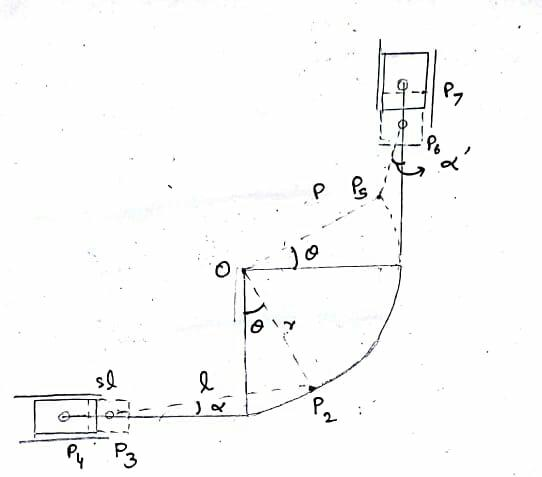
\includegraphics[scale=0.5]{bell}
		\caption{Bell Crank Mechanism1}
	\end{figure}
	\begin{eqnarray}
   p _{3}= r\sin{\theta}-l\cos{\alpha},-r\\
   p _{4}= r\sin{\theta}-l\cos{\alpha}-sl,-r\\
   p _{5}= r\cos{\theta},r\sin{\theta}\\
   p _{6}= r\cos{\theta}+l\sin{\alpha},r\sin{\theta}+l\cos{\alpha}\\
   p _{7}= r,r\sin{\theta}+l\cos{\alpha}+sl\\
	\end{eqnarray}
	\section{Animation in Matlab}
	\begin{figure}[H]
		\label{fig1}
		\centering
		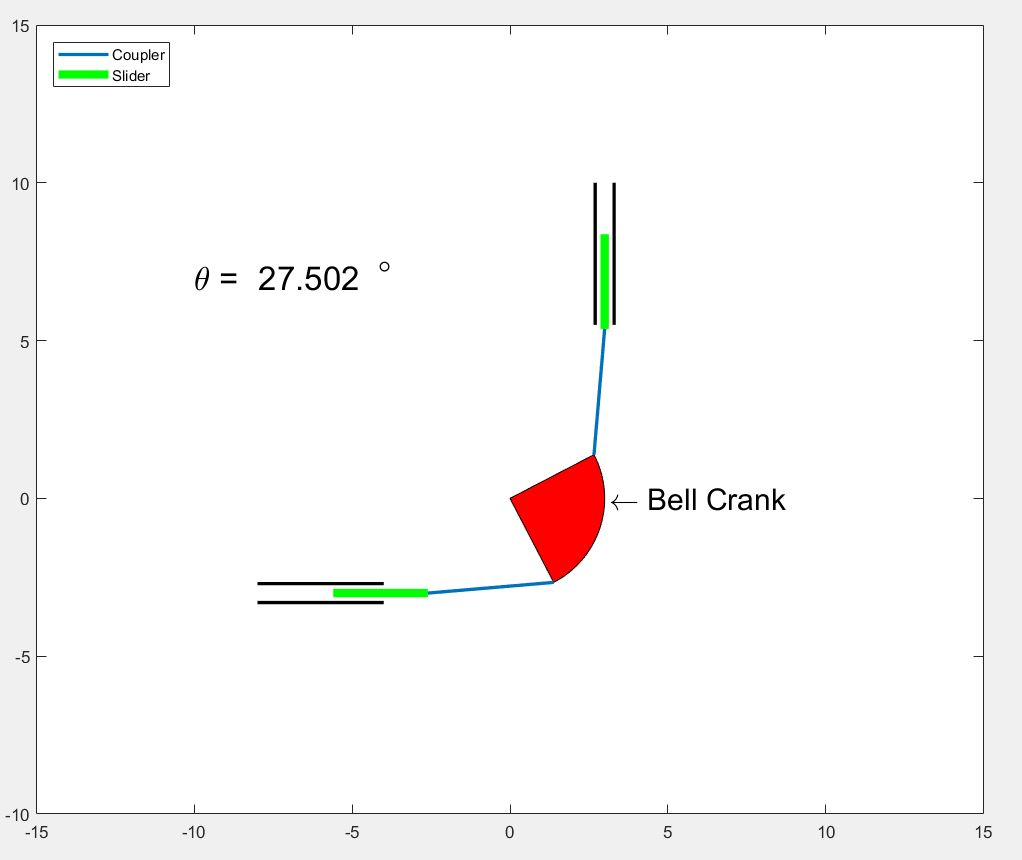
\includegraphics[scale=0.5]{crank}
		\caption{Bell Crank Mechanism2}
	\end{figure}
	\section{Application of Bell Crank Mechanism}
	\subsection{Aircraft}
	Bellcranks are often used in aircraft control systems to connect the pilot's controls to the control surfaces. For example: on light aircraft, the rudder often has a bellcrank whose pivot point is the rudder hinge. A cable connects the pilot's rudder pedal to one side of the bellcrank. When the pilot pushes on the rudder pedal, the rudder rotates on its hinge. The opposite rudder pedal is connected to the other end of the bellcrank to rotate the rudder in the opposite direction. Also referred to as a control horn.
	
	\subsection{Automative}
	Bellcranks are also seen in automotive applications, as part of the linkage connecting the throttle pedal to the carburetor, and connecting the brake pedal to the master brake cylinder. In vehicle suspensions, bellcranks are used in pushrod-style suspensions in automobiles or in the Christie suspension in tanks. Vertically-mounted suspensions may not be feasible in some vehicle designs due to space, aerodynamic, or other design constraints; bellcranks translate the vertical motion of the wheel into horizontal motion, allowing the suspension to be mounted transversely or longitudinally within the vehicle.
\end{document}